\documentclass[12pt]{article}
%%---------------------------------------------------------------------
% packages
% geometry
\usepackage{geometry}
% font
\usepackage{fontspec}
\defaultfontfeatures{Mapping=tex-text}  %%如果没有它,会有一些 tex 特殊字符无法正常使用,比如连字符。
\usepackage{xunicode,xltxtra}
\usepackage[BoldFont,SlantFont,CJKnumber,CJKchecksingle]{xeCJK}  % \CJKnumber{12345}: 一万二千三百四十五
\usepackage{CJKfntef}  %%实现对汉字加点、下划线等。
\usepackage{pifont}  % \ding{}
% math
\usepackage{amsmath,amsfonts,amssymb}
% color
\usepackage{color}
\usepackage{xcolor}
\definecolor{EYE}{RGB}{199,237,204}
\definecolor{FLY}{RGB}{128,0,128}
\definecolor{ZHY}{RGB}{139,0,255}
% graphics
\usepackage[americaninductors,europeanresistors]{circuitikz}
\usepackage{tikz}
\usetikzlibrary{positioning,arrows,shadows,shapes,calc,mindmap,trees,backgrounds}  % placements=positioning
\usepackage{graphicx}  % \includegraphics[]{}
\usepackage{subfigure}  %%图形或表格并排排列
% table
\usepackage{colortbl,dcolumn}  %% 彩色表格
\usepackage{multirow}
\usepackage{multicol}
\usepackage{booktabs}
% code
\usepackage{fancyvrb}
\usepackage{listings}
% title
\usepackage{titlesec}
% head/foot
\usepackage{fancyhdr}
% ref
\usepackage{hyperref}
% pagecolor
\usepackage[pagecolor={EYE}]{pagecolor}
% tightly-packed lists
\usepackage{mdwlist}
\usepackage{verbatim}%comment命令的注释包
\usepackage{styles/iplouccfg}
\usepackage{styles/zhfontcfg}
\usepackage{styles/iplouclistings}

%%---------------------------------------------------------------------
% settings
% geometry
\geometry{left=2cm,right=1cm,top=2cm,bottom=2cm}  %设置 上、左、下、右 页边距
\linespread{1.5} %行间距
% font
\setCJKmainfont{Adobe Kaiti Std}
%\setmainfont[BoldFont=Adobe Garamond Pro Bold]{Apple Garamond}  % 英文字体
%\setmainfont[BoldFont=Adobe Garamond Pro Bold,SmallCapsFont=Apple Garamond,SmallCapsFeatures={Scale=0.7}]{Apple Garamond}  %%苹果字体没有SmallCaps
\setCJKmonofont{Adobe Fangsong Std}
% graphics
\graphicspath{{figures/}}
\tikzset{
    % Define standard arrow tip
    >=stealth',
    % Define style for boxes
    punkt/.style={
           rectangle,
           rounded corners,
           draw=black, very thick,
           text width=6.5em,
           minimum height=2em,
           text centered},
    % Define arrow style
    pil/.style={
           ->,
           thick,
           shorten <=2pt,
           shorten >=2pt,},
    % Define style for FlyZhyBall
    FlyZhyBall/.style={
      circle,
      minimum size=6mm,
      inner sep=0.5pt,
      ball color=red!50!blue,
      text=white,},
    % Define style for FlyZhyRectangle
    FlyZhyRectangle/.style={
      rectangle,
      rounded corners,
      minimum size=6mm,
      ball color=red!50!blue,
      text=white,},
    % Define style for zhyfly
    zhyfly/.style={
      rectangle,
      rounded corners,
      minimum size=6mm,
      ball color=red!25!blue,
      text=white,},
    % Define style for new rectangle
    nrectangle/.style={
      rectangle,
      draw=#1!50,
      fill=#1!20,
      minimum size=5mm,
      inner sep=0.1pt,}
}
\ctikzset{
  bipoles/length=.8cm
}
% code
\lstnewenvironment{VHDLcode}[1][]{%
  \lstset{
    basicstyle=\footnotesize\ttfamily\color{black},%
    columns=flexible,%
    framexleftmargin=.7mm,frame=shadowbox,%
    rulesepcolor=\color{blue},%
%    frame=single,%
    backgroundcolor=\color{yellow!20},%
    xleftmargin=1.2\fboxsep,%
    xrightmargin=.7\fboxsep,%
    numbers=left,numberstyle=\tiny\color{blue},%
    numberblanklines=false,numbersep=7pt,%
    language=VHDL%
    }\lstset{#1}}{}
\lstnewenvironment{VHDLmiddle}[1][]{%
  \lstset{
    basicstyle=\scriptsize\ttfamily\color{black},%
    columns=flexible,%
    framexleftmargin=.7mm,frame=shadowbox,%
    rulesepcolor=\color{blue},%
%    frame=single,%
    backgroundcolor=\color{yellow!20},%
    xleftmargin=1.2\fboxsep,%
    xrightmargin=.7\fboxsep,%
    numbers=left,numberstyle=\tiny\color{blue},%
    numberblanklines=false,numbersep=7pt,%
    language=VHDL%
    }\lstset{#1}}{}
\lstnewenvironment{VHDLsmall}[1][]{%
  \lstset{
    basicstyle=\tiny\ttfamily\color{black},%
    columns=flexible,%
    framexleftmargin=.7mm,frame=shadowbox,%
    rulesepcolor=\color{blue},%
%    frame=single,%
    backgroundcolor=\color{yellow!20},%
    xleftmargin=1.2\fboxsep,%
    xrightmargin=.7\fboxsep,%
    numbers=left,numberstyle=\tiny\color{blue},%
    numberblanklines=false,numbersep=7pt,%
    language=VHDL%
    }\lstset{#1}}{}
% pdf
\hypersetup{pdfauthor={Haiyong Zheng},%
            pdftitle={Title},%
            CJKbookmarks=true,%
            bookmarksnumbered=true,%
            bookmarksopen=false,%
            plainpages=false,%
            colorlinks=true,%
            citecolor=green,%
            filecolor=magenta,%
            linkcolor=cyan,%red(default)
            urlcolor=cyan}
% section
%http://tex.stackexchange.com/questions/34288/how-to-place-a-shaded-box-around-a-section-label-and-name
\newcommand\titlebar{%
\tikz[baseline,trim left=3.1cm,trim right=3cm] {
    \fill [cyan!25] (2.5cm,-1ex) rectangle (\textwidth+3.1cm,2.5ex);
    \node [
        fill=cyan!60!white,
        anchor= base east,
        rounded rectangle,
        minimum height=3.5ex] at (3cm,0) {
        \textbf{\thesection.}
    };
}%
}
\titleformat{\section}{\Large\bf\color{blue}}{\titlebar}{0.1cm}{}
% head/foot
\setlength{\headheight}{15pt}
\pagestyle{fancy}
\fancyhf{}
%\lhead{\color{black!50!green}2014年秋季学期}
\chead{\color{black!50!green}Matlab安装}
%\rhead{\color{black!50!green}通信电子电路}
\lfoot{\color{blue!50!green}常琳(整理)}
%\cfoot{\color{blue!50!green}\href{http://vision.ouc.edu.cn/~zhenghaiyong}{CVBIOUC}}
\rfoot{\color{blue!50!green}$\cdot$\ \thepage\ $\cdot$}
\renewcommand{\headrulewidth}{0.4pt}
\renewcommand{\footrulewidth}{0.4pt}

%%---------------------------------------------------------------------
\begin{document}
%%---------------------------------------------------------------------
%%---------------------------------------------------------------------
% \titlepage
\title{\vspace{-2em}Matlab安装\vspace{-0.7em}}
\author{常琳(整理)}
\date{\vspace{-0.7em}2015年8月\vspace{-0.7em}}
%%---------------------------------------------------------------------
\maketitle\thispagestyle{fancy}
%%---------------------------------------------------------------------
\maketitle
\tableofcontents 
%---------------------------------------------------------------------

\section{安装}

\begin{enumerate}

\item 挂载iso文件

sudo  mount  -o  loop  路径Mathworks.Matlab.R2012a.UNIX.iso  /mnt  

\item 进入挂载目录

cd  /mnt

\item 安装

sudo  ./install

\item 出现图形化安装界面,破解说明在挂载目录下面的  crack  文件夹,建议安装到/opt/matlab目录下

\item 安装完成后,可以用用命令行打开matlab

sudo  /opt/matlab/bin/matlab

\item 解决The  desktop  configuration  was  not  saved  successfully
问题的关键就在于Permission  Denied,因此解决方法就是给目录和文件加权限,
代码:

sudo  chmod  a+w  -R  ~/.matlab

这一步也可以以后用到的时候写

\end{enumerate}

\section{创建快捷方式}

\begin{enumerate}
\item 将附件里的  matlab.desktop  文件放在  /usr/share/applications  下,图片  matlab.png  放在  /usr/share/icons  下

可以使用sudo  cp,也可以使用命令:

sudo  nautilus

进入文件管理器临时使用root权限,否则在用户账户下面没有权限在除  /home  之外的其他目录进行删除复制等操作。

\item 建立软链接使快捷方式生效

代码:

sudo  ln  -s  /opt/matlab/bin/matlab    /usr/bin/matlab

\end{enumerate}

\section{解决中文乱码问题}

\begin{enumerate}

\item 字体显示美化  进入Matlab,从菜单打开:Files->preferences,打开Fonts页,把右边最下面的复选框Use  antialising  to  smooth  desktop  fonts选中,重启MATLAB,字体显示的效果就很好了.

\item MATLAB使用自带的Java运行环境,根据CPU架构的不同,相对应的字体配置文件路径为:

32位版本  /usr/local/matlab/sys/java/jre/glnx86/jre/lib/fontconfig.properties

64位版本  /usr/local/matlab/sys/java/jre/glnxa64/jre/lib/fontconfig.properties

下面以64位版本为例进行配置

\item 进入字体配置文件目录

代码:

cd  /opt/matlab/sys/java/jre/glnx86/jre/lib

如果fontconfig.properties文件不存在,可以从fontconfig.properties.src复制一个。代码:

sudo  cp  fontconfig.properties.src  fontconfig.properties

效果图如图\ref{fig:1}
\begin{figure}[!htb] %插图
\centering
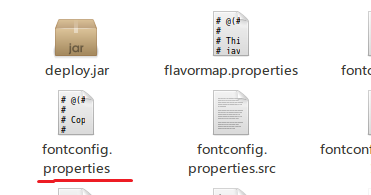
\includegraphics[width=0.5\textwidth]{1.png}
\caption{效果图一}
\label{fig:1}
\end{figure}

\item 字体可直接用系统自带的文泉驿即wqy文件夹,没有自己拷上。

修改JRE的字体配置文件,打开配置文件:

代码:

  sudo  gedit  fontconfig.properties

加入中文字体定义,在version=1下面一行输入

allfonts.chinese-arphic1=-misc-simsun-medium-r-normal--0-0-0-0-p-0-iso10646-1

接着指明中文字体路径,在allfonts.chinese-arphic1行后回车另起一行,输入中文字体文件的完整路径:

filename.-misc-simsun-medium-r-normal--0-0-0-0-p-0-iso10646-1=/usr/share/fonts/truetype/wqy/wqy-microhei.ttc

效果图如图\ref{fig:2}

\begin{figure}[!htb] %插图
\centering
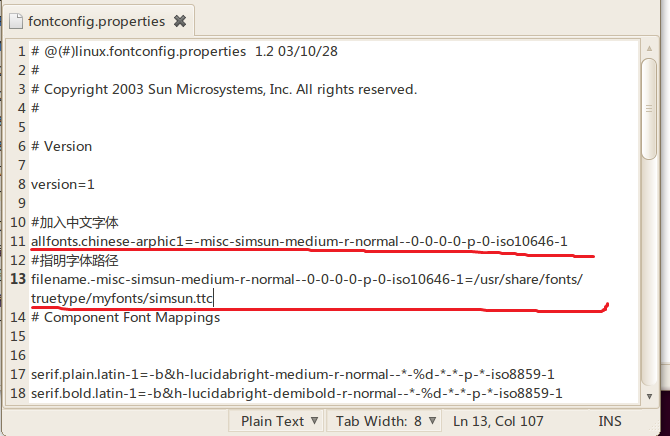
\includegraphics[width=0.5\textwidth]{2.png}
\caption{效果图二}
\label{fig:2}
\end{figure}


\item 修改字体搜索,  接着在此配置文件中查找  sequence.allfonts  行。如果其后的sequence开头的行中有:  chinese-arphics1,  可以略过此步;否则在其后面加入一行:  sequence.fallback=chinese-arphic1

 效果图如图\ref{fig:3}
\begin{figure}[!htb] %插图
\centering
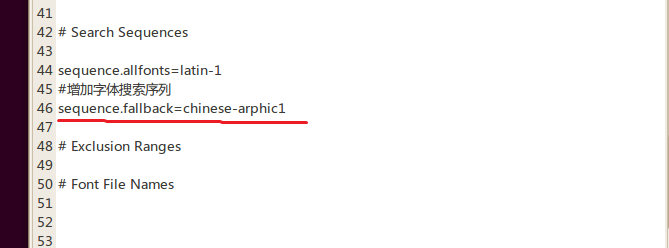
\includegraphics[width=0.5\textwidth]{3.png}
\caption{效果图三}
\label{fig:3}
\end{figure}


\end{enumerate}

完成。

参考网站:

\url{http://forum.ubuntu.org.cn/viewtopic.php?t=373776}


\end{document}


